% fig_fourpoints.tex -- written 2026-11-02 08:23 CET (from paper/siamnews/fig1.tex). Four points on a line at 0, 1, 5, 6;
% H0 barcode 1, 1, 4 = minimum spanning tree edges; two bars are nearest-neighbour distances, one is the gap.
% Line and barcode share one scale. \input inside a figure environment (no preamble).
\definecolor{fpV}{HTML}{D55E00}\definecolor{fpB}{HTML}{0072B2}%
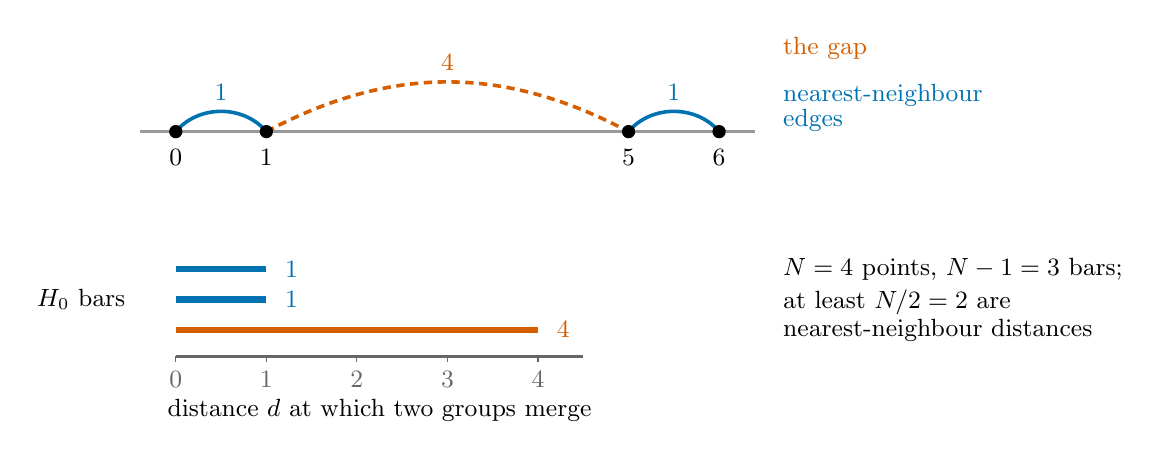
\begin{tikzpicture}[x=1.15cm, y=0.85cm, font=\small]
  \draw[black!40, line width=1pt] (-0.4,0) -- (6.4,0);
  \foreach \p in {0,1,5,6} { \draw[black!40] (\p,-0.08) -- (\p,0.08); \node[below=3pt] at (\p,0) {$\p$}; }
  \draw[fpB, line width=1.3pt] (0,0) to[bend left=50] node[above] {1} (1,0);
  \draw[fpB, line width=1.3pt] (5,0) to[bend left=50] node[above] {1} (6,0);
  \draw[fpV, line width=1.3pt, densely dashed] (1,0) to[bend left=28] node[above] {4} (5,0);
  \foreach \p in {0,1,5,6} \fill (\p,0) circle (2.4pt);
  \node[anchor=west, align=left, fpB] at (6.6,0.35) {nearest-neighbour\\[-2pt]edges};
  \node[anchor=west, fpV] at (6.6,1.25) {the gap};
  \begin{scope}[yshift=-1.75cm]
    \node[anchor=east] at (-0.45,-0.45) {$H_0$ bars};
    \draw[fpB, line width=2.2pt] (0,0) -- (1,0);       \node[anchor=west, fpB] at (1.1,0) {1};
    \draw[fpB, line width=2.2pt] (0,-0.45) -- (1,-0.45); \node[anchor=west, fpB] at (1.1,-0.45) {1};
    \draw[fpV, line width=2.2pt] (0,-0.9) -- (4,-0.9);   \node[anchor=west, fpV] at (4.1,-0.9) {4};
    \draw[black!60, line width=1pt] (0,-1.3) -- (4.5,-1.3);
    \foreach \v in {0,1,2,3,4} { \draw[black!60] (\v,-1.3) -- (\v,-1.38) node[below] {$\v$}; }
    \node[below] at (2.25,-1.8) {distance $d$ at which two groups merge};
    \node[anchor=west, align=left] at (6.6,-0.45) {$N=4$ points, $N-1=3$ bars;\\[1pt]at least $N/2=2$ are\\[-1pt]nearest-neighbour distances};
  \end{scope}
\end{tikzpicture}%
